\begin{frame}{Quiz 2}
	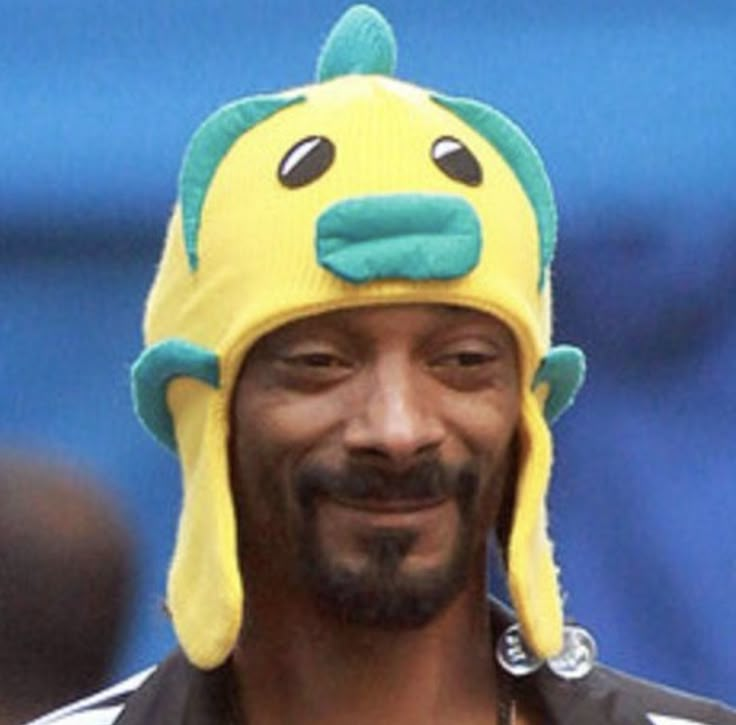
\includegraphics[width=0.5\textwidth]{images/snoophat.jpeg}
\end{frame}
%
%nextframe
\begin{frame}
	\begin{enumerate}
		\item Implemente el método \textbf{enqueue} que agrega un nodo
			a la cola (este método no retorna nada).
		\item Impemente el método \textbf{dequeue} que remueve el primer
			nodo de la cola y retorna el valor entero almacenado en
			ese nodo.
		\item Construya nodo por nodo la cola dada a continuación.
			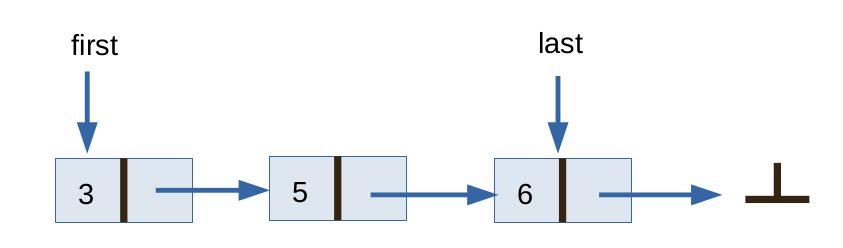
\includegraphics[width=0.75\textwidth]{images/queueQuiz2.png}
	\end{enumerate}
\end{frame}
